% Created by tikzDevice version 0.12.3.1 on 2021-01-15 17:47:56
% !TEX encoding = UTF-8 Unicode
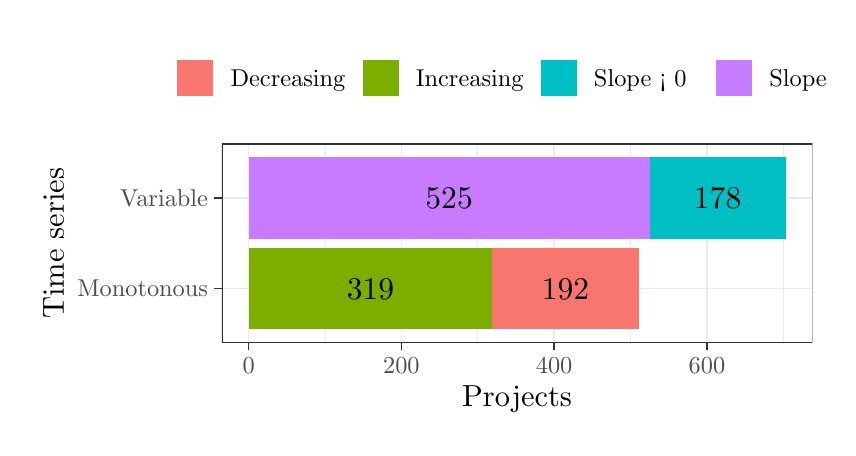
\begin{tikzpicture}[x=1pt,y=1pt]
\definecolor{fillColor}{RGB}{255,255,255}
\path[use as bounding box,fill=fillColor,fill opacity=0.00] (0,0) rectangle (289.08,144.54);
\begin{scope}
\path[clip] (  0.00,  0.00) rectangle (289.08,144.54);
\definecolor{drawColor}{RGB}{255,255,255}
\definecolor{fillColor}{RGB}{255,255,255}

\path[draw=drawColor,line width= 0.6pt,line join=round,line cap=round,fill=fillColor] (  0.00, -0.00) rectangle (289.08,144.54);
\end{scope}
\begin{scope}
\path[clip] ( 70.13, 30.69) rectangle (283.58,102.59);
\definecolor{fillColor}{RGB}{255,255,255}

\path[fill=fillColor] ( 70.13, 30.69) rectangle (283.58,102.59);
\definecolor{drawColor}{gray}{0.92}

\path[draw=drawColor,line width= 0.3pt,line join=round] (107.43, 30.69) --
	(107.43,102.59);

\path[draw=drawColor,line width= 0.3pt,line join=round] (162.64, 30.69) --
	(162.64,102.59);

\path[draw=drawColor,line width= 0.3pt,line join=round] (217.84, 30.69) --
	(217.84,102.59);

\path[draw=drawColor,line width= 0.3pt,line join=round] (273.05, 30.69) --
	(273.05,102.59);

\path[draw=drawColor,line width= 0.6pt,line join=round] ( 70.13, 50.29) --
	(283.58, 50.29);

\path[draw=drawColor,line width= 0.6pt,line join=round] ( 70.13, 82.98) --
	(283.58, 82.98);

\path[draw=drawColor,line width= 0.6pt,line join=round] ( 79.83, 30.69) --
	( 79.83,102.59);

\path[draw=drawColor,line width= 0.6pt,line join=round] (135.04, 30.69) --
	(135.04,102.59);

\path[draw=drawColor,line width= 0.6pt,line join=round] (190.24, 30.69) --
	(190.24,102.59);

\path[draw=drawColor,line width= 0.6pt,line join=round] (245.45, 30.69) --
	(245.45,102.59);
\definecolor{fillColor}{RGB}{124,174,0}

\path[fill=fillColor] ( 79.83, 35.59) rectangle (167.88, 65.00);
\definecolor{fillColor}{RGB}{248,118,109}

\path[fill=fillColor] (167.88, 35.59) rectangle (220.88, 65.00);
\definecolor{fillColor}{RGB}{199,124,255}

\path[fill=fillColor] ( 79.83, 68.27) rectangle (224.75, 97.68);
\definecolor{fillColor}{RGB}{0,191,196}

\path[fill=fillColor] (224.75, 68.27) rectangle (273.88, 97.68);
\definecolor{drawColor}{RGB}{0,0,0}

\node[text=drawColor,anchor=base,inner sep=0pt, outer sep=0pt, scale=  1.14] at (123.86, 46.38) {319};

\node[text=drawColor,anchor=base,inner sep=0pt, outer sep=0pt, scale=  1.14] at (194.38, 46.38) {192};

\node[text=drawColor,anchor=base,inner sep=0pt, outer sep=0pt, scale=  1.14] at (152.29, 79.06) {525};

\node[text=drawColor,anchor=base,inner sep=0pt, outer sep=0pt, scale=  1.14] at (249.31, 79.06) {178};
\definecolor{drawColor}{gray}{0.20}

\path[draw=drawColor,line width= 0.6pt,line join=round,line cap=round] ( 70.13, 30.69) rectangle (283.58,102.59);
\end{scope}
\begin{scope}
\path[clip] (  0.00,  0.00) rectangle (289.08,144.54);
\definecolor{drawColor}{gray}{0.30}

\node[text=drawColor,anchor=base east,inner sep=0pt, outer sep=0pt, scale=  0.88] at ( 65.18, 47.26) {Monotonous};

\node[text=drawColor,anchor=base east,inner sep=0pt, outer sep=0pt, scale=  0.88] at ( 65.18, 79.95) {Variable};
\end{scope}
\begin{scope}
\path[clip] (  0.00,  0.00) rectangle (289.08,144.54);
\definecolor{drawColor}{gray}{0.20}

\path[draw=drawColor,line width= 0.6pt,line join=round] ( 67.38, 50.29) --
	( 70.13, 50.29);

\path[draw=drawColor,line width= 0.6pt,line join=round] ( 67.38, 82.98) --
	( 70.13, 82.98);
\end{scope}
\begin{scope}
\path[clip] (  0.00,  0.00) rectangle (289.08,144.54);
\definecolor{drawColor}{gray}{0.20}

\path[draw=drawColor,line width= 0.6pt,line join=round] ( 79.83, 27.94) --
	( 79.83, 30.69);

\path[draw=drawColor,line width= 0.6pt,line join=round] (135.04, 27.94) --
	(135.04, 30.69);

\path[draw=drawColor,line width= 0.6pt,line join=round] (190.24, 27.94) --
	(190.24, 30.69);

\path[draw=drawColor,line width= 0.6pt,line join=round] (245.45, 27.94) --
	(245.45, 30.69);
\end{scope}
\begin{scope}
\path[clip] (  0.00,  0.00) rectangle (289.08,144.54);
\definecolor{drawColor}{gray}{0.30}

\node[text=drawColor,anchor=base,inner sep=0pt, outer sep=0pt, scale=  0.88] at ( 79.83, 19.68) {0};

\node[text=drawColor,anchor=base,inner sep=0pt, outer sep=0pt, scale=  0.88] at (135.04, 19.68) {200};

\node[text=drawColor,anchor=base,inner sep=0pt, outer sep=0pt, scale=  0.88] at (190.24, 19.68) {400};

\node[text=drawColor,anchor=base,inner sep=0pt, outer sep=0pt, scale=  0.88] at (245.45, 19.68) {600};
\end{scope}
\begin{scope}
\path[clip] (  0.00,  0.00) rectangle (289.08,144.54);
\definecolor{drawColor}{RGB}{0,0,0}

\node[text=drawColor,anchor=base,inner sep=0pt, outer sep=0pt, scale=  1.10] at (176.85,  7.64) {Projects};
\end{scope}
\begin{scope}
\path[clip] (  0.00,  0.00) rectangle (289.08,144.54);
\definecolor{drawColor}{RGB}{0,0,0}

\node[text=drawColor,rotate= 90.00,anchor=base,inner sep=0pt, outer sep=0pt, scale=  1.10] at ( 13.08, 66.64) {Time series};
\end{scope}
\begin{scope}
\path[clip] (  0.00,  0.00) rectangle (289.08,144.54);
\definecolor{fillColor}{RGB}{255,255,255}

\path[fill=fillColor] ( 42.35,113.59) rectangle (311.36,139.04);
\end{scope}
\begin{scope}
\path[clip] (  0.00,  0.00) rectangle (289.08,144.54);
\definecolor{fillColor}{RGB}{255,255,255}

\path[fill=fillColor] ( 53.35,119.09) rectangle ( 67.81,133.54);
\end{scope}
\begin{scope}
\path[clip] (  0.00,  0.00) rectangle (289.08,144.54);
\definecolor{fillColor}{RGB}{248,118,109}

\path[fill=fillColor] ( 54.06,119.80) rectangle ( 67.10,132.83);
\end{scope}
\begin{scope}
\path[clip] (  0.00,  0.00) rectangle (289.08,144.54);
\definecolor{fillColor}{RGB}{255,255,255}

\path[fill=fillColor] (120.30,119.09) rectangle (134.76,133.54);
\end{scope}
\begin{scope}
\path[clip] (  0.00,  0.00) rectangle (289.08,144.54);
\definecolor{fillColor}{RGB}{124,174,0}

\path[fill=fillColor] (121.02,119.80) rectangle (134.05,132.83);
\end{scope}
\begin{scope}
\path[clip] (  0.00,  0.00) rectangle (289.08,144.54);
\definecolor{fillColor}{RGB}{255,255,255}

\path[fill=fillColor] (184.69,119.09) rectangle (199.14,133.54);
\end{scope}
\begin{scope}
\path[clip] (  0.00,  0.00) rectangle (289.08,144.54);
\definecolor{fillColor}{RGB}{0,191,196}

\path[fill=fillColor] (185.40,119.80) rectangle (198.43,132.83);
\end{scope}
\begin{scope}
\path[clip] (  0.00,  0.00) rectangle (289.08,144.54);
\definecolor{fillColor}{RGB}{255,255,255}

\path[fill=fillColor] (248.02,119.09) rectangle (262.48,133.54);
\end{scope}
\begin{scope}
\path[clip] (  0.00,  0.00) rectangle (289.08,144.54);
\definecolor{fillColor}{RGB}{199,124,255}

\path[fill=fillColor] (248.73,119.80) rectangle (261.77,132.83);
\end{scope}
\begin{scope}
\path[clip] (  0.00,  0.00) rectangle (289.08,144.54);
\definecolor{drawColor}{RGB}{0,0,0}

\node[text=drawColor,anchor=base west,inner sep=0pt, outer sep=0pt, scale=  0.88] at ( 73.31,123.28) {Decreasing};
\end{scope}
\begin{scope}
\path[clip] (  0.00,  0.00) rectangle (289.08,144.54);
\definecolor{drawColor}{RGB}{0,0,0}

\node[text=drawColor,anchor=base west,inner sep=0pt, outer sep=0pt, scale=  0.88] at (140.26,123.28) {Increasing};
\end{scope}
\begin{scope}
\path[clip] (  0.00,  0.00) rectangle (289.08,144.54);
\definecolor{drawColor}{RGB}{0,0,0}

\node[text=drawColor,anchor=base west,inner sep=0pt, outer sep=0pt, scale=  0.88] at (204.64,123.28) {Slope < 0};
\end{scope}
\begin{scope}
\path[clip] (  0.00,  0.00) rectangle (289.08,144.54);
\definecolor{drawColor}{RGB}{0,0,0}

\node[text=drawColor,anchor=base west,inner sep=0pt, outer sep=0pt, scale=  0.88] at (267.98,123.28) {Slope > 0};
\end{scope}
\end{tikzpicture}
